\documentclass[13pt,oneside]{book}
\usepackage[utf8]{inputenc}
\usepackage{url}
\usepackage{graphicx}

\usepackage{geometry}
\geometry{a4paper, left=20mm, right=20mm, top=20mm, bottom=20mm}
\usepackage[margin=1.2in]{geometry}
\usepackage[toc,page]{appendix}
\usepackage{graphicx}
\usepackage{natbib}
\usepackage{lipsum}
\usepackage{caption}

\begin{document}

\captionsetup[figure]{margin=1.5cm,font=small,labelfont={bf},name={Figure},labelsep=colon,textfont={it}}
\captionsetup[table]{margin=1.5cm,font=small,labelfont={bf},name={Table},labelsep=colon,textfont={it}}
\setlipsumdefault{1}

\begin{titlepage}
\begin{center}
{\LARGE College Of Engineering Trivandrum}\\[3cm]
\linespread{1.2}\huge {\bfseries Application Software Development Lab}\\[3cm]
\linespread{1}

\includegraphics[width=5cm]{img/emblem.jpeg}\\[3cm]
{\Large GOKUL K\\ S5  CSE \\ Roll No:21\\ TVE18CS021 }\\[1cm]


\textit{ }\\[2cm]
Department of Computer Science\\[0.2cm]
\today
\end{center}

\end{titlepage}

\newpage

\begin{frame}{}
    \centering
    \hspace*{-0.5cm}
    $\vcenter{\hbox{
\includegraphics[width=1.5cm]{img/emblem.jpeg}}}$
    $\vcenter{\resizebox{0.95\textwidth}{!}{
        \begin{tabular}{c}
             CS333 - Application Software Development Lab $\cdot$ 2020 $\cdot$   \\
             \hline 
        \end{tabular}
    }}$
\end{frame}
\section*{Cycle 2}
\section*{Expt 3}
\begin{center}
    \Large{Triggers and Exception Handling}
\end{center}

\section*{Aim}
\large To study PL/SQL trigger and exception handling.

\section*{Expiriment}
\begin{itemize}
	\item
	Creating tables
	 
	Syntax:
	\begin{verbatim}
		CREATE TABLE customer_details (
			cust_id INT UNIQUE,
			cust_name VARCHAR(25),
			address VARCHAR(30)
		);
		
		CREATE TABLE emp_details (
			empid INT UNIQUE,
			empname VARCHAR(25),
			SALARY INT
		);
		
		CREATE TABLE cust_count (
			count_row INT
		);
	
	\end{verbatim}
	
	
	\item
	Create a trigger whenever a new record is inserted in the customer details
	table.

	Syntax:
	\begin{verbatim}
CREATE OR REPLACE FUNCTION customer_details_insert() RETURNS TRIGGER AS
$customer_details_insert$
	BEGIN
		RAISE NOTICE 'Row inserted';
		RETURN NEW;
	END;
$customer_details_insert$
LANGUAGE plpgsql;

CREATE TRIGGER customer_details_insert
AFTER INSERT ON customer_details
	FOR EACH STATEMENT EXECUTE PROCEDURE customer_details_insert();
	
	\end{verbatim}
	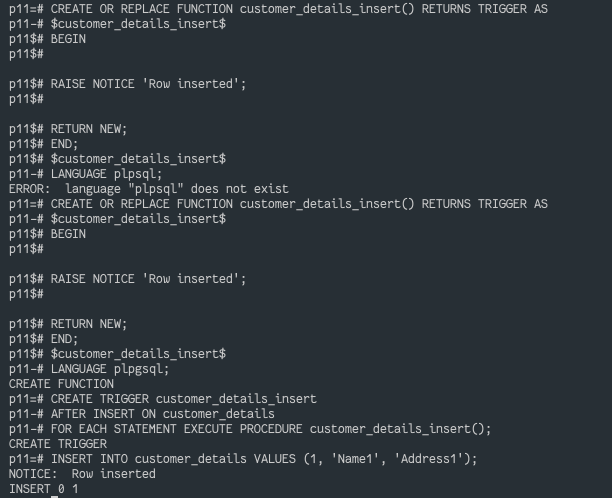
\includegraphics[]{img/p10/ss1.png}
	
	
	\item
	Create a trigger to display a message when a user enters a value >20000
	in the salary field of emp details table.
	 
	Syntax:
	\begin{verbatim}
		CREATE OR REPLACE FUNCTION employee_salary_check() RETURNS trigger AS $employee_salary$
		BEGIN
			IF NEW.salary > 20000 
			THEN
				RAISE NOTICE 'Inserted employee % has salary greater 20000', NEW.empname;
			END IF;
			RETURN NEW;
		END;
	$employee_salary$ LANGUAGE plpgsql;
	
	CREATE TRIGGER employee_salary AFTER INSERT OR UPDATE ON emp_details
		FOR EACH ROW EXECUTE PROCEDURE employee_salary_check();

	\end{verbatim}
	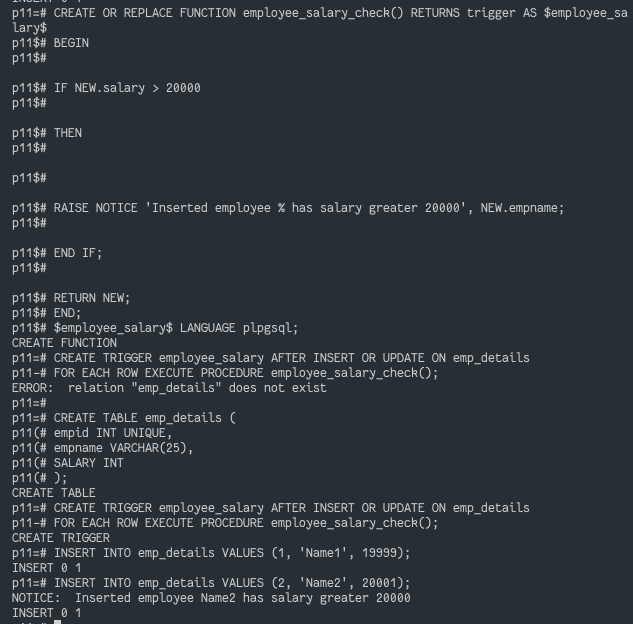
\includegraphics[]{img/p10/ss2.png}
	
	
	\item
	Create a trigger w.r.tcustomer detailstable.
Increment the value of count row (in cust count table) whenever a new tuple is 
inserted and decrement the value of count row when a tuple is deleted.
	 
	Syntax:
	\begin{verbatim}
CREATE OR REPLACE FUNCTION cust_count() RETURNS trigger 
AS $cust_count$ DECLARE
	count INT;
	BEGIN
		SELECT * FROM cust_count INTO count;
		IF (TG_OP = 'DELETE' AND count != 0) THEN
			UPDATE cust_count SET count_row=count_row-1;
		ELSIF (TG_OP = 'INSERT') THEN
			UPDATE cust_count SET count_row=count_row+1;
		END IF;
		RETURN NEW;
	END;
$cust_count$ LANGUAGE plpgsql;

CREATE TRIGGER cust_count_change
AFTER INSERT OR DELETE ON customer_details
	FOR EACH ROW EXECUTE PROCEDURE cust_count();
	
	\end{verbatim}
	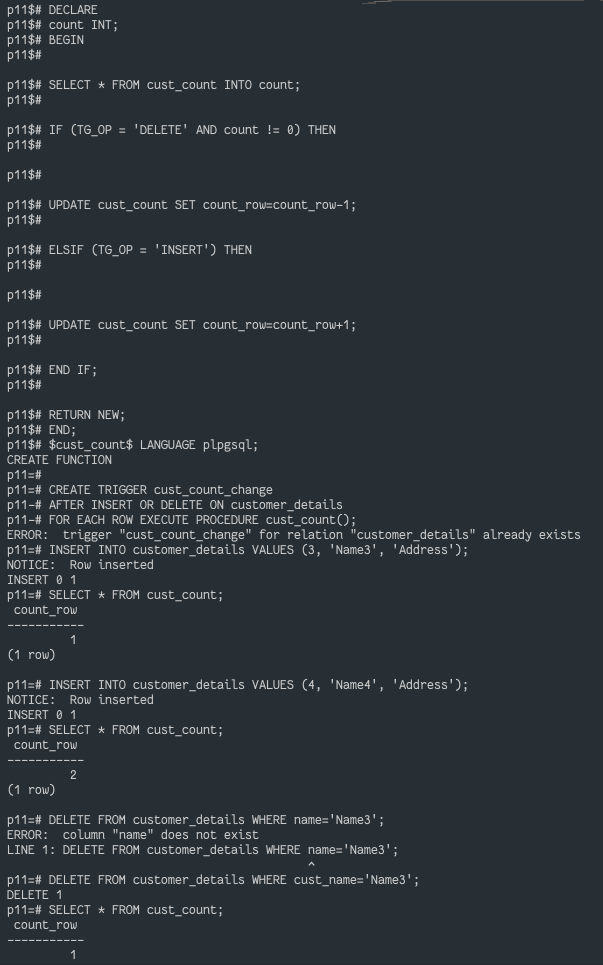
\includegraphics[]{img/p10/ss3.png}
	
	
	\item
	Create a trigger to insert the deleted rows from emp details to another
	table and updated rows to another table. ( Create the tables deleted and
	updatedT )

	Syntax:
	\begin{verbatim}
		CREATE TABLE deleted (
			empid INT UNIQUE,
			empname VARCHAR(25),
			SALARY INT
		);
		
		CREATE TABLE updated (
			empid INT UNIQUE,
			empname VARCHAR(25),
			SALARY INT
		);
		
		CREATE OR REPLACE FUNCTION delete_update() RETURNS trigger AS $delete_update$
		BEGIN
			IF(TG_OP = 'DELETE') THEN
				INSERT INTO deleted VALUES (OLD.empid, OLD.empname, OLD.salary);
			ELSIF(TG_OP = 'UPDATE') THEN
				INSERT INTO updated VALUES (OLD.empid, OLD.empname, OLD.salary);
			END IF;
			RETURN NEW;
		END;
		$delete_update$ LANGUAGE plpgsql;
		
		CREATE TRIGGER delete_update
		AFTER UPDATE OR DELETE ON emp_details
			FOR EACH ROW EXECUTE PROCEDURE delete_update();

		\end{verbatim}
	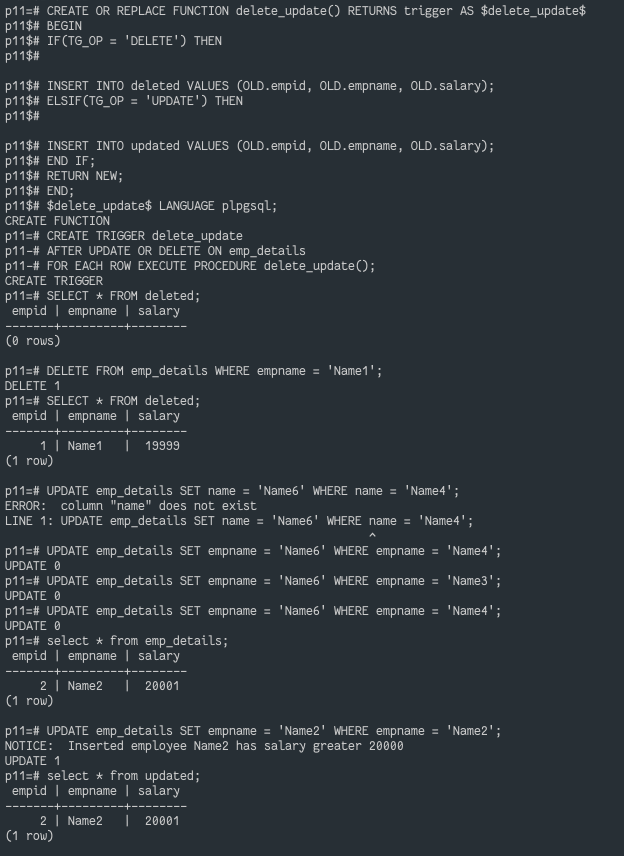
\includegraphics[]{img/p10/ss4.png}
	
	
	\item
	Write a PL/SQL to show divide by zero exception

	Syntax:
	\begin{verbatim}
		CREATE OR REPLACE FUNCTION div(a INT, b INT) RETURNS INT AS 
		$$
		DECLARE
			result INT;
			BEGIN
				IF b = 0 THEN
					RAISE EXCEPTION 'DIVIDE BY ZERO';
				ELSE
					result = a/b;
					RETURN result;
				END IF;
			END;
		$$
		LANGUAGE plpgsql;
	
	\end{verbatim}
	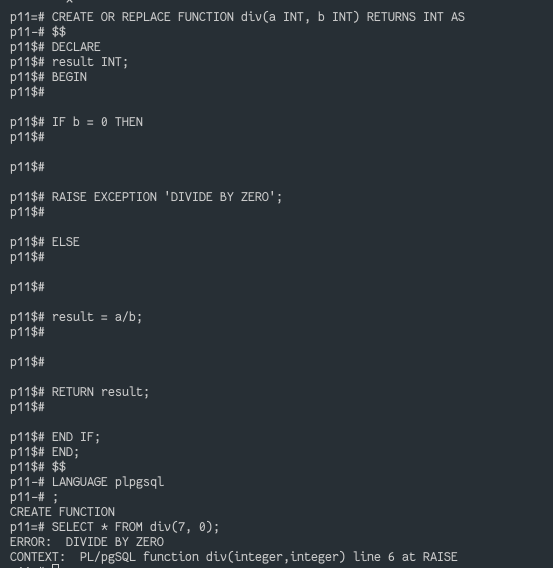
\includegraphics[]{img/p10/ss5.png}
	
	
	\item
	Write a PL/SQL to show no data found exception
	 
	Syntax:
	\begin{verbatim}
		CREATE OR REPLACE FUNCTION get_salary(id INT) RETURNS INT as
		$$
		DECLARE
			result INT;
		BEGIN
			SELECT salary INTO result FROM emp_details WHERE empid=id;
			IF RESULT IS NULL THEN
				RAISE EXCEPTION 'No data foudn';
			ELSE
				RETURN result;
			END IF;
		END;
		$$
		LANGUAGE plpgsql;
	
	\end{verbatim}
	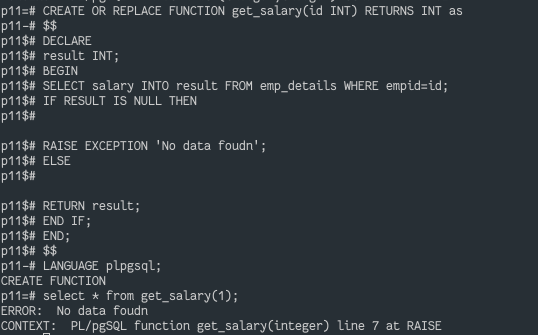
\includegraphics[]{img/p10/ss6.png}
	
	
	\item
	Create a table with ebill(cname,prevreading,currreading). If prevreading
= currreading then raise an exception Data Entry Error
	 
	Syntax:
	\begin{verbatim}
		CREATE TABLE ebill (
			cname VARCHAR(20),
			preread INT,
			curread INT
		);
		
		CREATE OR REPLACE FUNCTION check_reading() RETURNS TRIGGER AS
		$checkread$
		BEGIN
			IF NEW.preread=NEW.curread THEN
				RAISE EXCEPTION 'Data error % %' ,NEW.preread,NEW.curread;
			ELSE
				RAISE NOTICE 'Data entered';
			END IF;
			RETURN NEW;
		END;
		$checkread$
		LANGUAGE plpgsql;
		
		CREATE TRIGGER check_reading
		BEFORE INSERT ON ebill
		FOR EACH ROW EXECUTE PROCEDURE check_reading();
	
	\end{verbatim}
	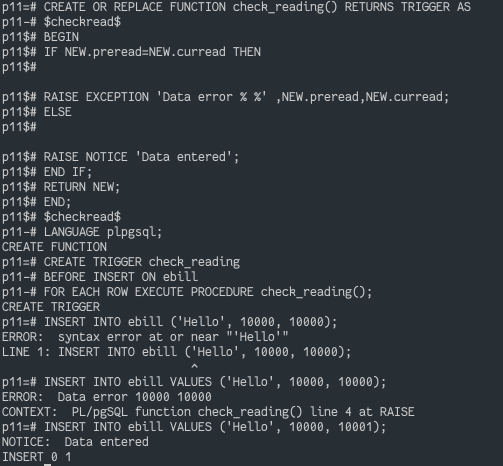
\includegraphics[]{img/p10/ss7.png}
	

	
\end{itemize}
\section*{Result}
	Triggers and exception handling is executed and their output
	is verified in a PostgreSQL environment.
\end{document}